\documentclass[11pt]{amsart}
\usepackage{geometry}                % See geometry.pdf to learn the layout options. There are lots.
\geometry{letterpaper}                   % ... or a4paper or a5paper or ... 
%\geometry{landscape}                % Activate for for rotated page geometry
%\usepackage[parfill]{parskip}    % Activate to begin paragraphs with an empty line rather than an indent
\usepackage{graphicx}
\usepackage{parskip}
\usepackage{amssymb}
\usepackage{epstopdf}
\DeclareGraphicsRule{.tif}{png}{.png}{`convert #1 `dirname #1`/`basename #1 .tif`.png}

\title{Brief Article}
\author{The Author}
%\date{}                                           % Activate to display a given date or no date

\begin{document}
\maketitle
%\section{}
%\subsection{}
\setlength{\parindent}{1cm}
\section {Objective}
The purpose of this practical is to design and implement a standalone image annotation application that satisfies the following User requirements:

\begin{itemize}
\item  User friendly way of opening an image
\item  User friendly way of editing, adding and deleting image labels and selecting corresponding image
areas
\item  User friendly way of saving and loading the label set
\item The interface is easy to use
\item The interface allow fast processing of large number of images
\item The layout uses affordances to guide users.
\end{itemize}



  
\section {Obtaining data}
 Before designing and  defining the functional specification of our system, we first  analysed the existing system \(``Label Me ``\) to gain insights on what areas has this web based tool  been successful and on what areas has it failed to cope the usability requirements.

Upon careful analysis, we have found the following usability problems associated with ``Label Me" tool:
\begin{enumerate}
\item  For each annotated polygon the tool provides a different color. Although this allows  the users to distinguish between landmarks, the use of different colors at times make it difficult  for a user to locate a particular landmark \textbf{instantly} when he/ she places his cursor on a particular label situated on the right side of the screen.
\item It is not clear on first sight on how to undo a step or sequence of steps  when annotating a   landmark in the current image.  Renaming the \emph{ Erase} button to \emph{Undo} will definitely provide better navigation control for a first time  user. Plus, the user has no means to redo some of his previous steps
\item One of the main disadvantages that we have found is that the tool does not provide any means for a user to save his work and  progress to a different image. The inability to move between different projects hence makes the tool less appealing to potential users.
\item Another flaw that we encountered  during our analysis is in the use of the \emph{Zoom Buttons}. The user is not allowed to zoom any portion of the annotated image when he/she is in the process of creating a polygon. This restriction is totally redundant and only puts more unnecessary on how the user can interact with the tool.
\item To edit a polygon, the user is required to click in a specific region inside the polygon. Since the region is not specified, needless time and effort has to be spent on locating this region. In addition, the tool does not provide any options to \textbf{ add new points} or \text{remove points} from an existing saved polygon.
\end{enumerate}


Apart from the cons , the ``Label Me "  provides a user with a range of functionalities :
\begin {itemize}
\item  It allows user to label particular landmarks in an image.
\item  The landmarks are annotated with different colors, thus making it easily to differentiate between different landmarks.
\item  As soon as a user puts  his cursor on a particular label, the polygon associated with the label is highlighted ,hence making it easy to identify that particular landmark.
\item The editing tools provided by `Label Me " allows  the user to adjust the shape and location of the polygons.
\end{itemize}



\section {Design  and  Implementation Process}

The design of our interface consists of a bottom up approach. To be more elaborate, we have divided the design and implementation stages into 3 layers(show in figure 1). 
\begin{figure}
\centerline{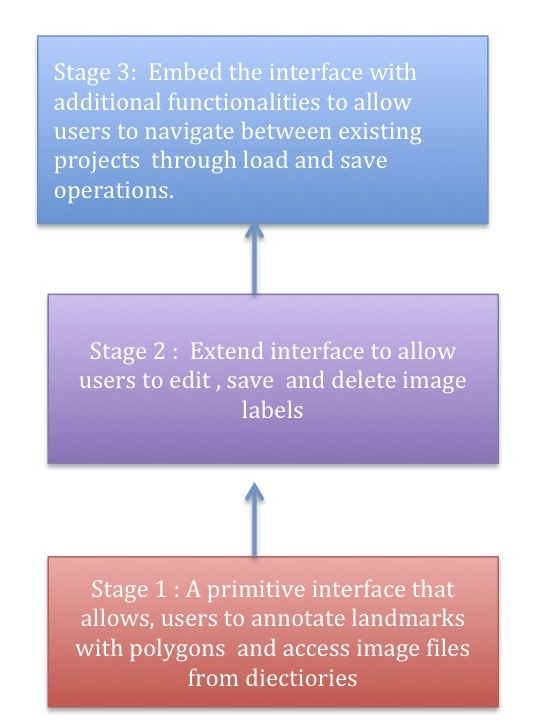
\includegraphics[height=100mm]{layers.jpg}}
\caption{}
\label{DM}
\end{figure}


Hence,  our aim  has been to develop an  initial primitive interface and then  add higher functionalities at each stage/layer hence extending the range of user capabilities . In our methodology, prior to the implementation process of each layer, we have applied  task analysis and phototype evaluation to evaluate the practicality of our designs.
We have attempted to follow  a combination of Shneiderman' and Neilsans HCi design rules for all the 3 stages. The rules that we have taken into consideration are as follows:
\begin{enumerate}
\item  Enable frequent users to use shortcuts
\item  Offer informative feedback
\item Design dialogs to yield closure
\item  Offer error prevention and simple error handling
\item  Permit easy reversal of actions
\item Match between system and the real world
\item User control and freedom
\end{enumerate}



 


\end{document}  